\documentclass[11pt, english]{article}
\usepackage{graphicx}
\usepackage[colorlinks=true, linkcolor=blue]{hyperref}
\usepackage[english]{babel}
\selectlanguage{english}
\usepackage[utf8]{inputenc}
\usepackage[svgnames]{xcolor}

\usepackage{afterpage}
\usepackage{amsmath}
\usepackage{amsfonts}
\usepackage{amssymb}
\usepackage{algorithm}
\usepackage{algorithmic}

\pagestyle{plain}

\definecolor{dkgreen}{rgb}{0,0.6,0}
\definecolor{gray}{rgb}{0.5,0.5,0.5}
\definecolor{mauve}{rgb}{0.58,0,0.82}

\usepackage{here}

\textheight=21cm
\textwidth=16cm
%\topmargin=-1cm
\oddsidemargin=0cm
\parindent=0mm
\pagestyle{plain}

%%%%%%%%%%%%%%%%%%%%%%%%%%
%
%%%%%%%%%%%%%%%%%%%%%%%%%%

\usepackage{color}
\usepackage{ragged2e}

\begin{document}

\setlength\parskip{.3\baselineskip}
\begin{titlepage}

\begin{center}
\begin{figure}[htb]
\begin{center}

\includegraphics[width=8cm]{gsu_c_logo}
\end{center}
\end{figure}

\begin{Large}
\textbf{Georgia State University} \\
\end{Large}
Department of Computer Science \\
\vspace*{0.2in}
\begin{Large}
\textbf{title of report} \\
\end{Large}
\vspace*{0.3in}
\begin{large}
Ph.D Qualifier Report\\
\end{large}
\vspace*{0.3in}
\begin{large}
Xiulong Yang\\
\end{large}
\vspace*{0.3in}
\rule{80mm}{0.1mm}\\
\vspace*{0.1in}
\begin{large}
Committee:\\
\vspace*{0.1in}
Dr.(Chair), Dr., and Dr.\\
\end{large}
\end{center}
\end{titlepage}

\newcommand{\CC}{C\nolinebreak\hspace{-.05em}\raisebox{.4ex}{\tiny\bf +}\nolinebreak\hspace{-.10em}\raisebox{.4ex}{\tiny\bf +}}
\def\CC{{C\nolinebreak[4]\hspace{-.05em}\raisebox{.4ex}{\tiny\bf ++}}}

%----------------------------------------------------------------------------------------
%	Abstract Section
%----------------------------------------------------------------------------------------

\begin{abstract}
  The background.

  In this work, two XXX algorithms will be investigated, including A and B. Experiments show that they are good.

  \textbf{Key words:} Deep Learning, Machine Learning
    

\end{abstract}

\newpage

\[
\begin{matrix}
d_{11} & d_{12} & d_{13} & \dots & d_{1n}\\
  & d_{22} & d_{23} & \dots & d_{2n}\\
  &  & d_{33}       &\dots & d_{3n}\\
  &  &              &\ddots & \vdots\\
  &  &              &       & d_{nn}
\end{matrix}
\]

\tableofcontents
\newpage

%----------------------------------------------------------------------------------------
%	Introduction Section
%----------------------------------------------------------------------------------------

\section{Introduction}

Over the past few years, the issues have raised some what.

In this work, two selected papers "A" and "B" presented two approaches.

The outline of the report is as follows: In Section II,
we will review some related work of  . In Section III,  . The next method is then introduced in Section III. Finally,conclusions and future work in Section V and VI.
\newpage
%----------------------------------------------------------------------------------------
%	background Section
%----------------------------------------------------------------------------------------

\section{Related Work}

I guess this part is very important too.
\newpage

%----------------------------------------------------------------------------------------
%	paper1 Section
%----------------------------------------------------------------------------------------

\section{title}

\subsection{subsection}

a equation
$$
p(y=c|x, w) = softmax(f(x))
$$
. The $w$ is the parameters of a neural network, and $f$ is the output of the model. So for each input image, we can get a probability vector $p(y=c|x, w)$.

The authors evaluated the models on MNIST (\cite{mnist}), CIFAR-10 (\cite{cifar10}), a diabetic retinopathy dataset (\cite{retinopathy}) and ImageNet(\cite{resnet}). Shaded areas in the plots denote $\pm$ one standard deviation.


\begin{enumerate}
    \item MNIST: The network architecture for MNIST, referred to as “S-CNN”, contains two convolutional layers and one dense layer. It is the same as the Keras MNIST CNN implementation (\cite{keras_cnn}).
    \item CIFAR-10: The authors experiment a CNN model with four convolutional layers and one dense layer as the Keras CIFAR CNN implementation (\cite{keras_cnn}), which we refer to as “K-CNN”. 
    
    Additionally they also evaluate with DenseNet-121 (k = 12, with bottleneck), using the learning rate schedule as proposed in \cite{denseNet}. 
    \item diabetic retinopathy dataset: Details for the inceptionV3 architecture are described in section 4.5.
    \item ImageNet: ResNet-50\cite{resnet} is used in the experiments. The network is trained for 100 epochs without data augmentation using stochastic gradient descent. The initial learning rate of 0.1 is changed to 0.01 at epoch 50, and 0.001 at epoch 75. The initial 40,000 images are class-balanced.
\end{enumerate}

Figure.\ref{figure1} is show below:

\begin{figure}[ht!]
    \centering
    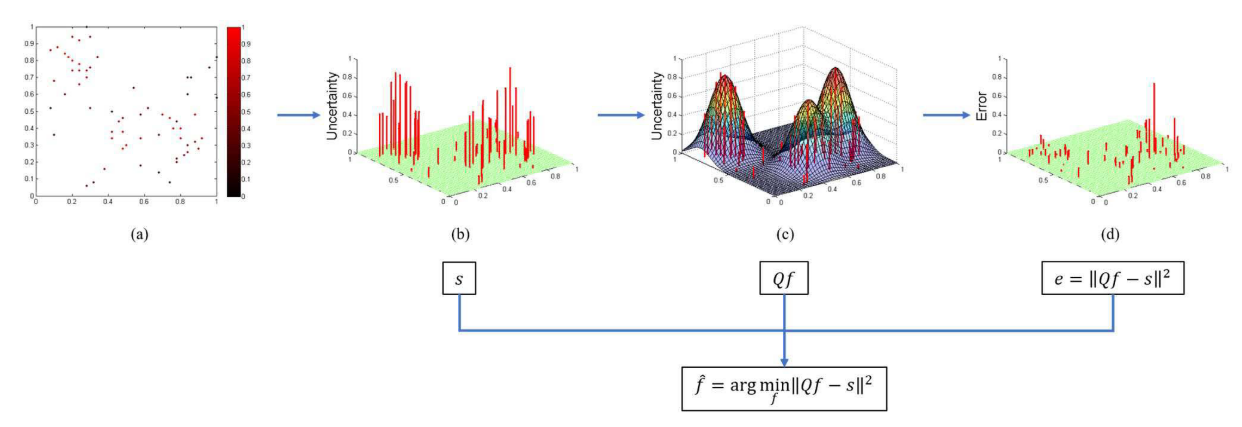
\includegraphics[width=15.4cm]{sparse_overview.png}
    \caption{overview}
    \label{figure1}
\end{figure}
\newpage
%----------------------------------------------------------------------------------------
%	paper2 Section
%----------------------------------------------------------------------------------------

\renewcommand{\algorithmicrequire}{\textbf{Input:}}
\renewcommand{\algorithmicensure}{\textbf{Output:}} 

\section{paper2's title}

\subsection{Motivation}

\begin{equation}
\begin{aligned} 
    \widehat{f} = & \operatorname{argmin}_{f} - f^{T} s + \frac{1}{2} f^{T} K f \\ 
    &\text{s.t.}\sum_{i=1}^{n}f_{i}=1,\quad f_{i}\geq0
\end{aligned}
\label{equ:max_div}
\end{equation}

\begin{algorithm}
\caption{SMGS}
\label{alg:gs}
\begin{algorithmic}
    \REQUIRE ~~\\
    original uncertainty values $s$, similarity matrix $Q$, \\
    labeled set $L$, unlabeled set $U$
    \STATE \textbf{Initialization:} Set $s^1 = s$
    \FOR{$t = 1:B_q$}
        \STATE Choose $k^t = arg \max_{j\in U} q^T_j s^t$ from $U$
        \STATE Compute $f_{k^t}$ by $$ f_{k^t} = arg \min_{f_{k^t}} ||f_{k^t} q_{k^t} - s^t||^2.$$
        \STATE Update the uncertainty values for the next iteration.
        \STATE using $$s^{t+1} = max(s^t - f_{k^t}, 0).$$
        \STATE Move sample index $k^t$ from $U$ to $L$.
    \ENDFOR
    \ENSURE ~~ updated labeled set L
\end{algorithmic}
    \label{code:SMGS}
\end{algorithm}



\begin{figure}[ht!]
    \centering
    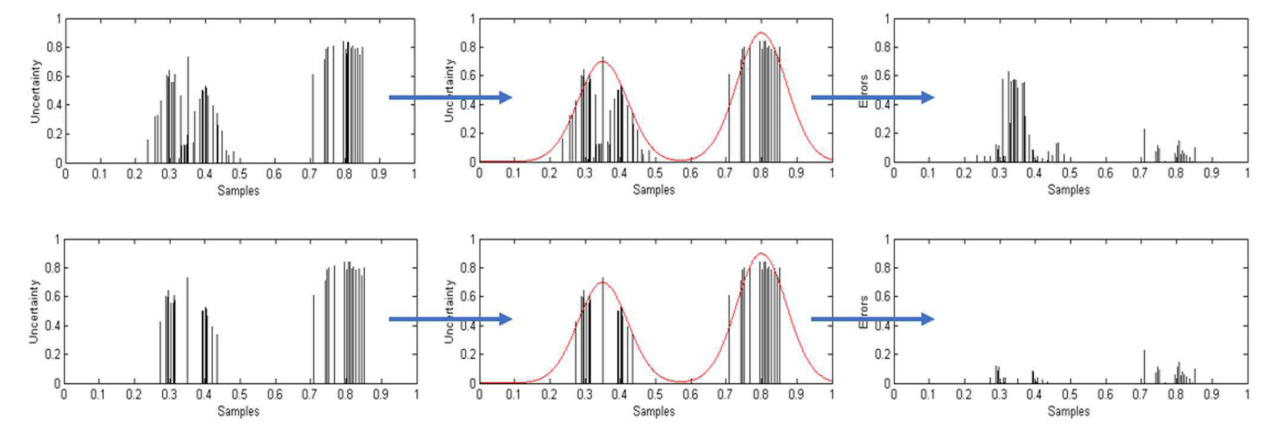
\includegraphics[width=10.4cm]{sparse_selective.png}
    \caption{The overview}
    \label{sparse_time}
\end{figure}

The Figure.\ref{sparse_time} shows the idea.
\newpage

%----------------------------------------------------------------------------------------
%   future work Section
%----------------------------------------------------------------------------------------
\section{Future Work}

Future is good

%----------------------------------------------------------------------------------------
%   Conclusion Section
%----------------------------------------------------------------------------------------
\section{Conclusion}

it's the conclusion

\newpage

\bibliographystyle{plain}
\bibliography{ref}

\end{document}
